\section{Moduł obsługi kontrahentów}
\singlespacing

\subsection{Zarządzanie danymi kontrahentów} 
\begin{usecase}
\addtitle{PU8}{Zarządzanie danymi kontrahentów} 
% Priorytet
\addfield{Priorytet:}{wysoki}
\addfield{Aktor główny:}{Użytkownik}
\additemizedfield{Warunki początkowe:}{
  \item Aktor został uwierzytelniony.
} 
\addscenario{Scenariusz główny:}{
	\item Aktor wybiera opcję przeglądania kontrahentów.
    \item System wyświetla listę kontrahentów.
}
\addfield{Wymagania funkcjonalne}{3. Zarządzanie danymi kontrahentów}
\end{usecase}

\begin{figure}[H]
  \centering
  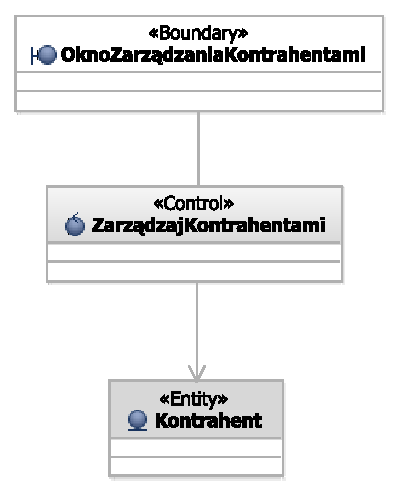
\includegraphics[angle=\ecbangle, scale=\ecbscale]{../img/usecase/pu8ecb.pdf}
  \caption{\ecbcaption8}
\end{figure}
\newpage %!!!!!!!!!!!!!!!!!!!!! RECZNA zmiana strony!
\begin{figure}[H]
  \centering
  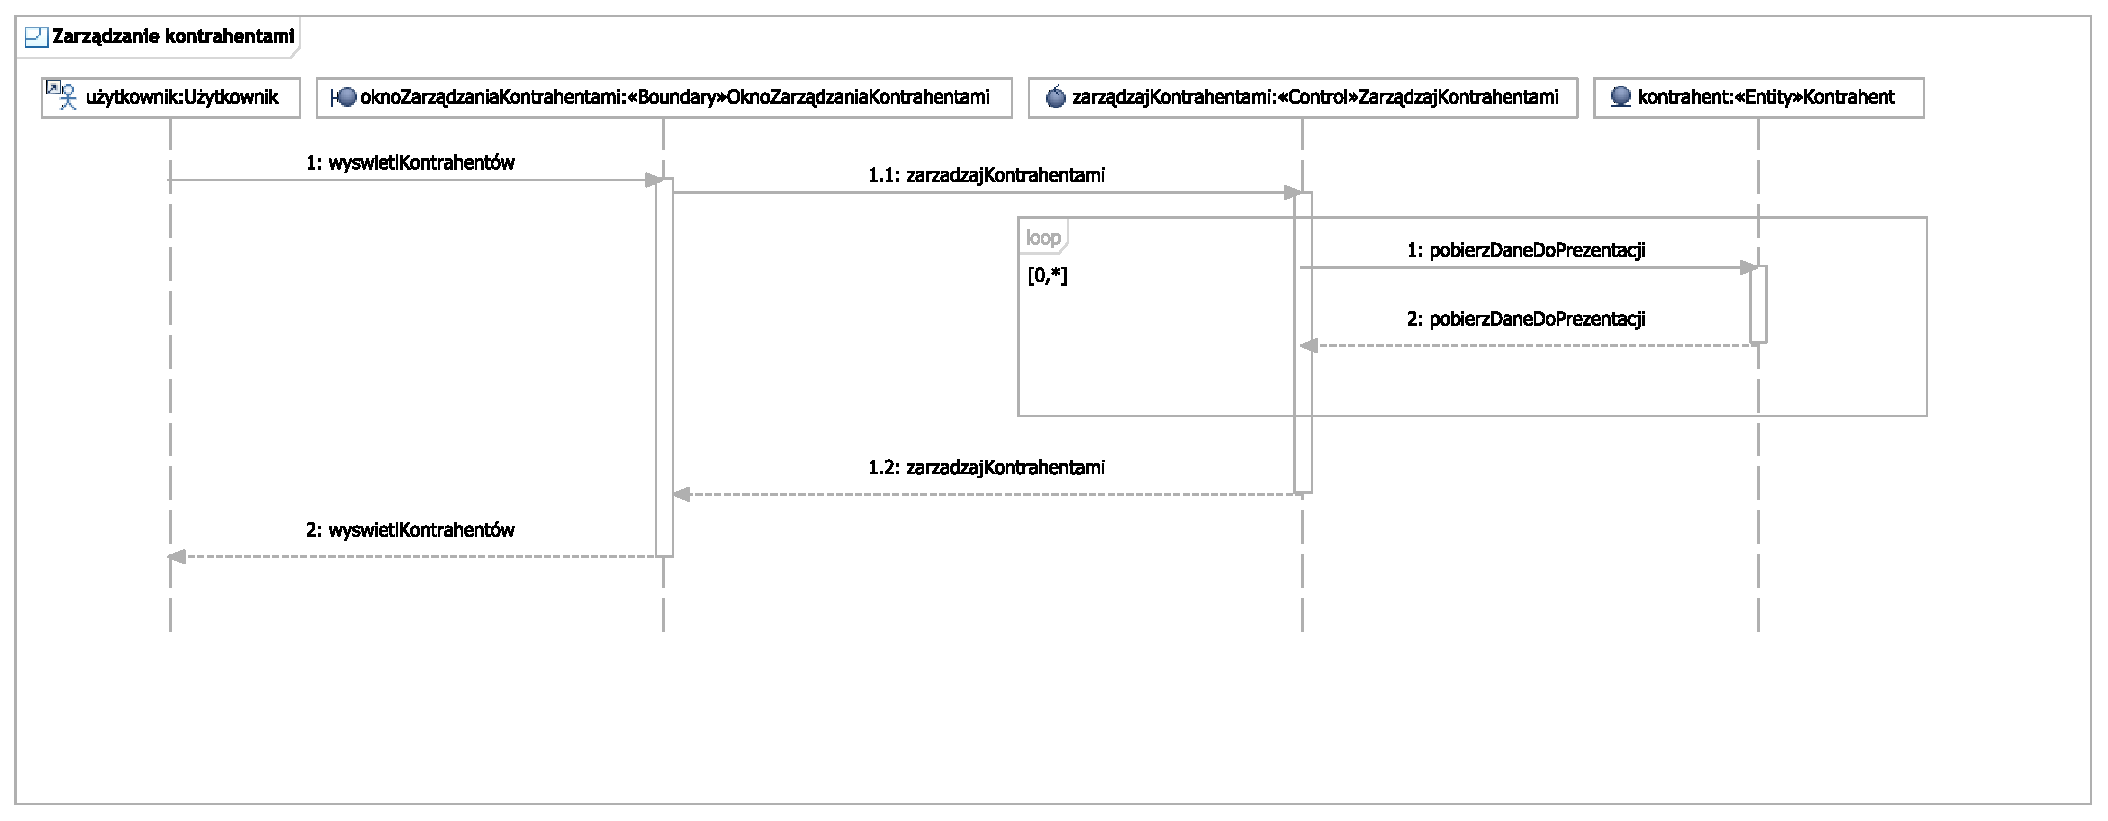
\includegraphics[angle=\seqangle, scale=0.45]{../img/usecase/pu8seq.pdf}
  \caption{\seqcaption8}
\end{figure}
\newpage

\subsection{Dodawanie kontrahentów}
\begin{usecase}
\addtitle{PU9}{Dodawanie kontrahenta} 
\addfield{Priorytet:}{wysoki}
\addfield{Aktor główny:}{Użytkownik}
\addfield{Rozszerza przypadki:}{PU8}
\additemizedfield{Warunki początkowe:}{
  \item Aktor został uwierzytelniony.
} 
\addfield{Warunki końcowe:}{Dane kontrahenta zostają zapisane w systemie}
\addscenario{Scenariusz główny:}{
	\item Aktor wybiera opcję dodania nowego kontrahenta.
    \item System wyświetla formularz umożliwiający wprowadzenie danych kontrahenta.
    \item Aktor wprowadza dane kontrahenta.
    \item Aktor zatwierdza wprowadzone dane.
    \item System sprawdza poprawność wprowadzonych danych.
    \item System zapisuje dane nowego kontrahenta.
    \item System wyświetla potwierdzenie wykonania operacji.
}
\addscenario{Scenariusz alternatywny:}{
	\item[6.a] Wprowadzono błędne dane
		\begin{enumerate}
		\item[1.--5.] Jak w scenariuszu głównym.
		\item[6.] System wyświetla komunikat informujący o wprowadzeniu błędnych danych.
		\item[7.] Powrót do punktu 3. scenariusza głównego.
		\end{enumerate}
}
\addfield{Wymagania funkcjonalne}{3. Zarządzanie danymi kontrahentów, 3.1 Dodawanie kontrahentów}
\end{usecase}

\begin{figure}[H]
  \centering
  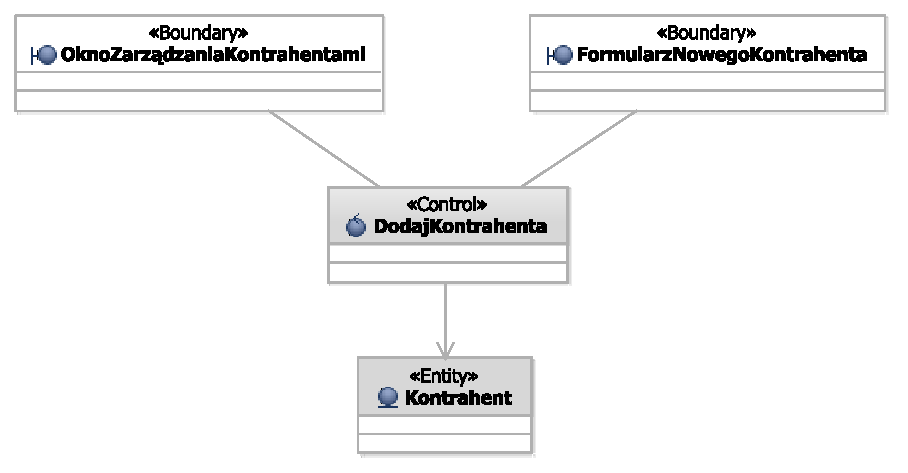
\includegraphics[angle=\ecbangle, scale=\ecbscale]{../img/usecase/pu9ecb.pdf}
  \caption{\ecbcaption9}
\end{figure}
\begin{figure}[H]
  \centering
  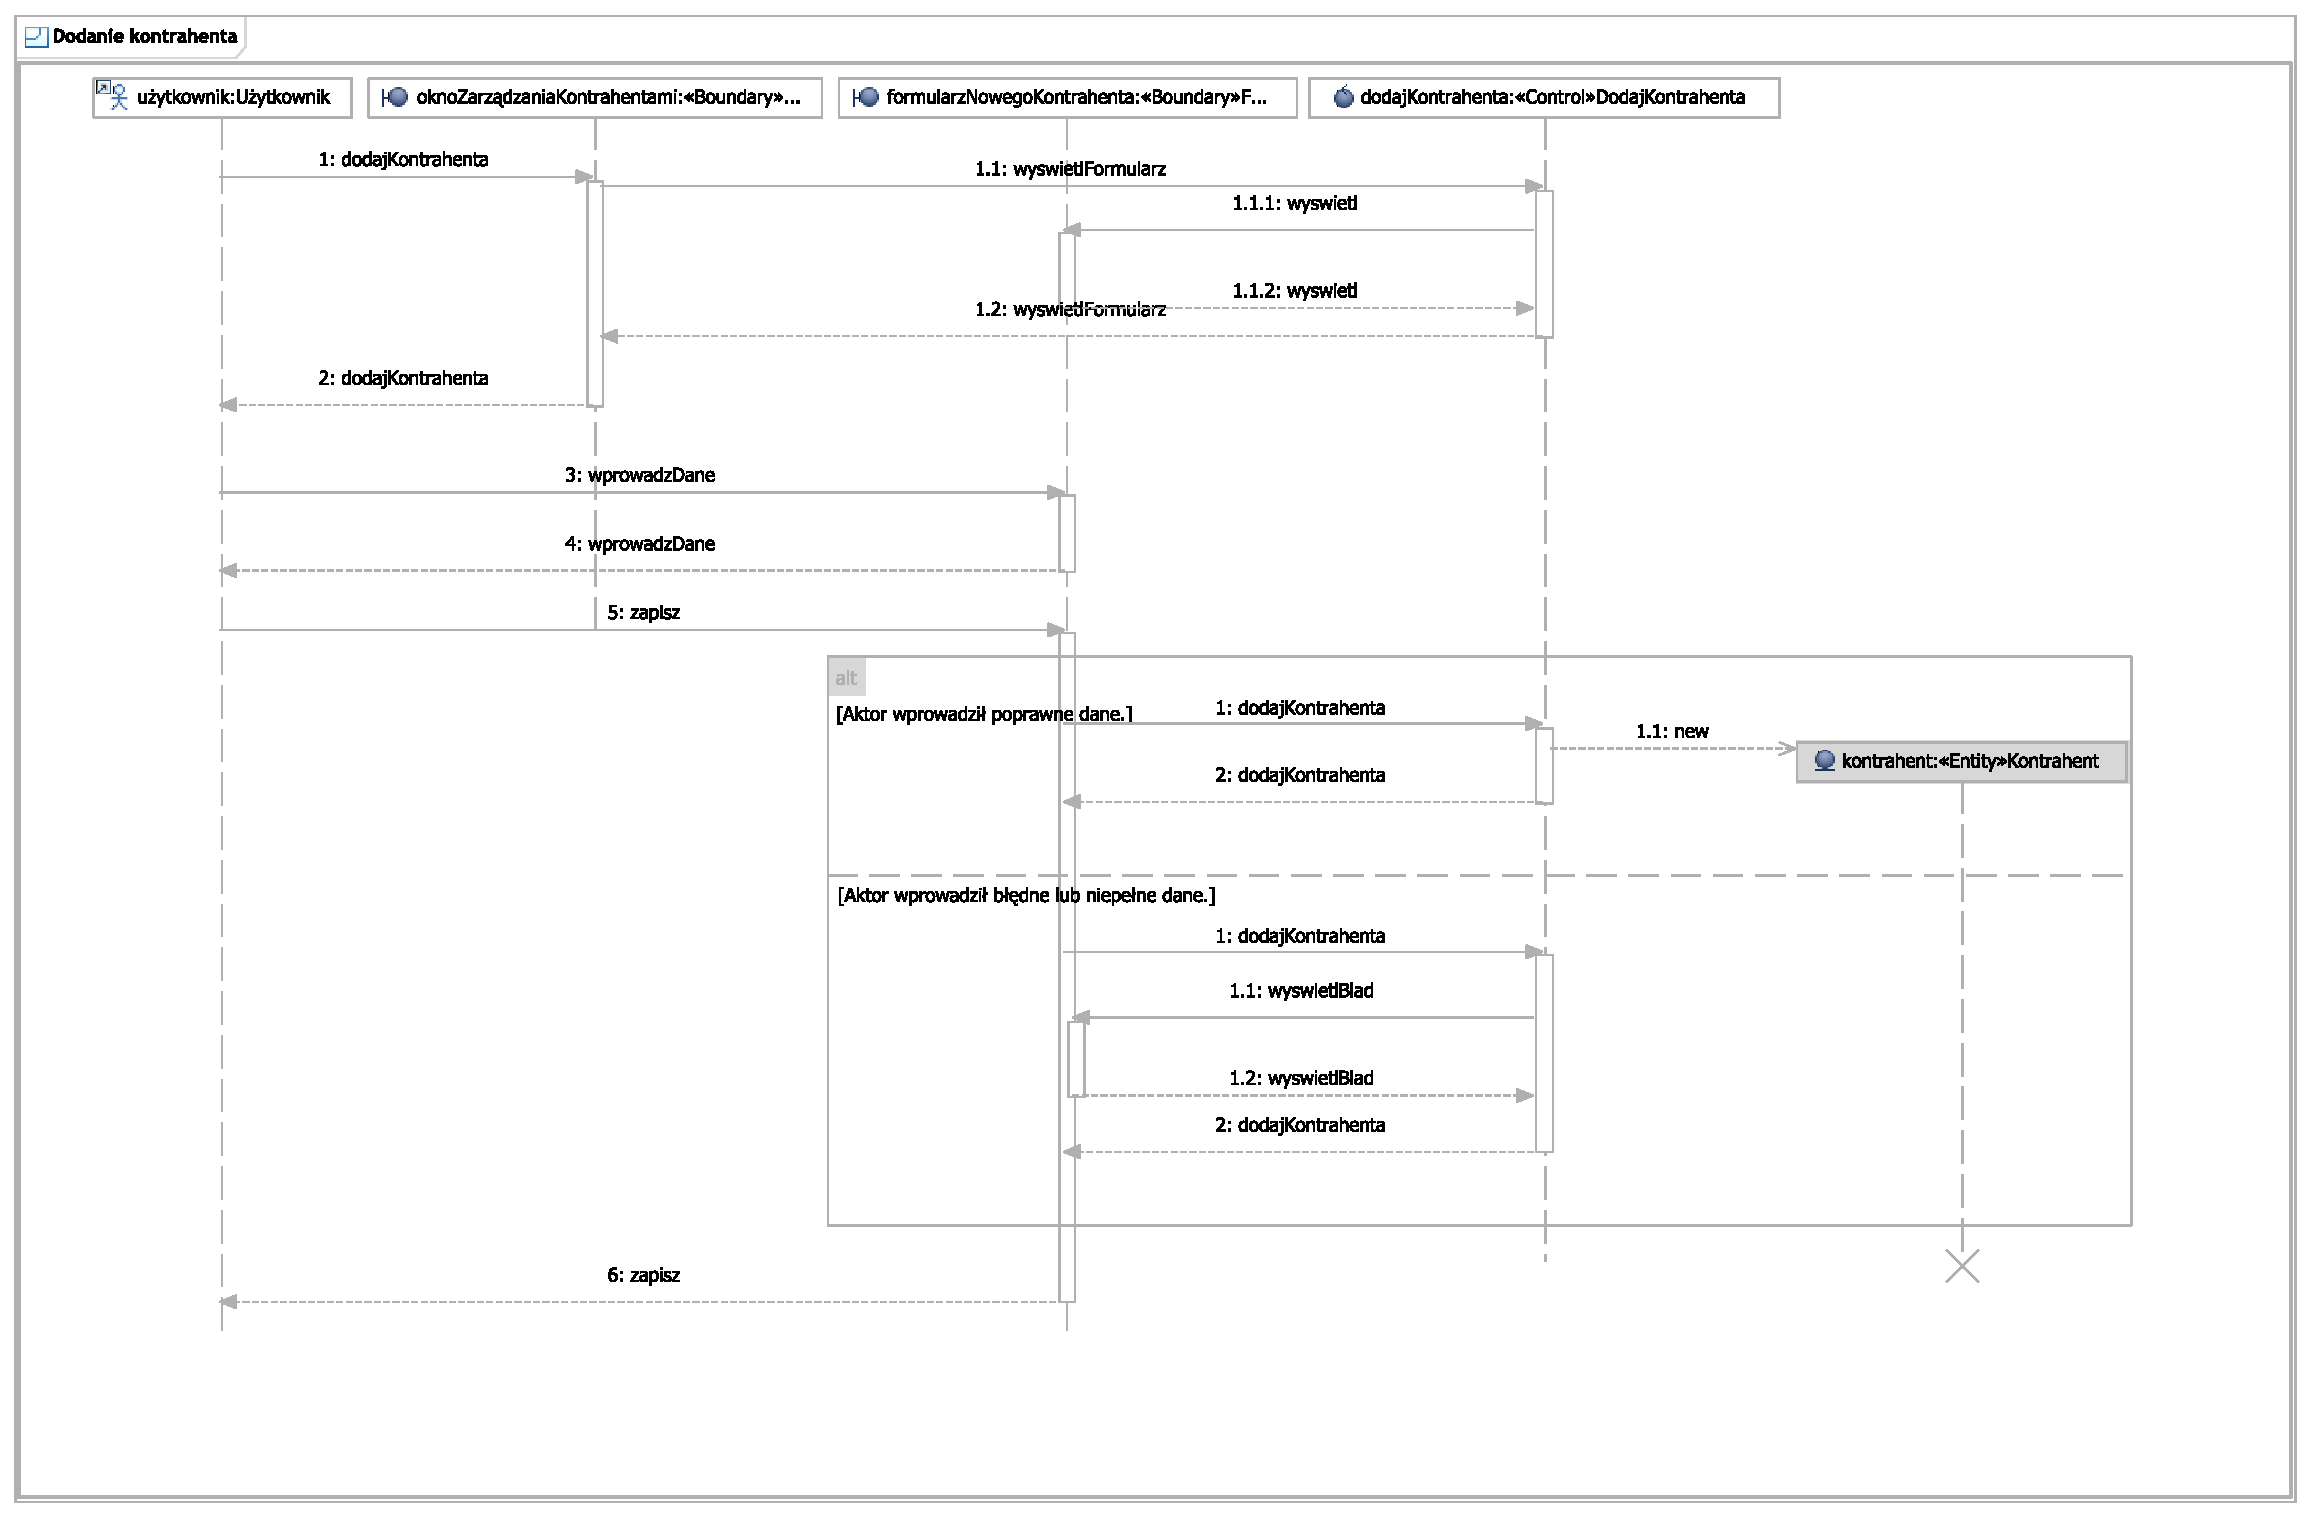
\includegraphics[angle=\seqangle, scale=\seqscalemin]{../img/usecase/pu9seq.pdf}
  \caption{\seqcaption9}
\end{figure}
\newpage

\subsection{Edycja danych kontrahentów}
\begin{usecase}
\addtitle{PU10}{Edycja danych kontrahenta} 
\addfield{Priorytet:}{wysoki}
\addfield{Aktor główny:}{Użytkownik}
\addfield{Rozszerza przypadki:}{PU8}
\additemizedfield{Warunki początkowe:}{
  \item Aktor został uwierzytelniony.
  \item W systemie istnieje co najmniej jeden kontrahent.
} 
\addfield{Warunki końcowe:}{Dane kontrahenta zostają zmienione w systemie}
\addscenario{Scenariusz główny:}{
	\item Aktor wybiera opcję edycji kontrahenta.
    \item System wyświetla formularz umożliwiający modyfikację danych kontrahenta.
    \item Aktor modyfikuje dane kontrahenta.
    \item Aktor zatwierdza wprowadzone zmiany.
    \item System sprawdza poprawność wprowadzonych danych.
    \item System zapisuje zmienione dane kontrahenta.
    \item System wyświetla potwierdzenie wykonania operacji.
}
\addscenario{Scenariusz alternatywny:}{
	\item[6.a] Wprowadzono błędne dane
		\begin{enumerate}
		\item[1.--5.] Jak w scenariuszu głównym.
		\item[6.] System wyświetla komunikat informujący o wprowadzeniu błędnych danych.
		\item[7.] Powrót do punktu 3. scenariusza głównego.
		\end{enumerate}
}
\addfield{Wymagania funkcjonalne}{3. Zarządzanie danymi kontrahentów, 3.2 Edycja danych kontrahentów}
\end{usecase}

\begin{figure}[H]
  \centering
  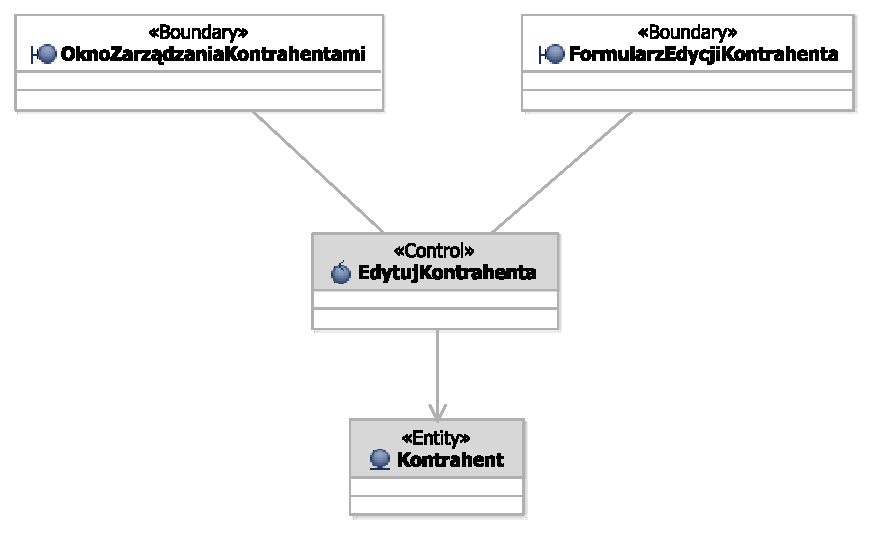
\includegraphics[angle=\ecbangle, scale=\ecbscale]{../img/usecase/pu10ecb.pdf}
  \caption{\ecbcaption10}
\end{figure}
\begin{figure}[H]
  \centering
  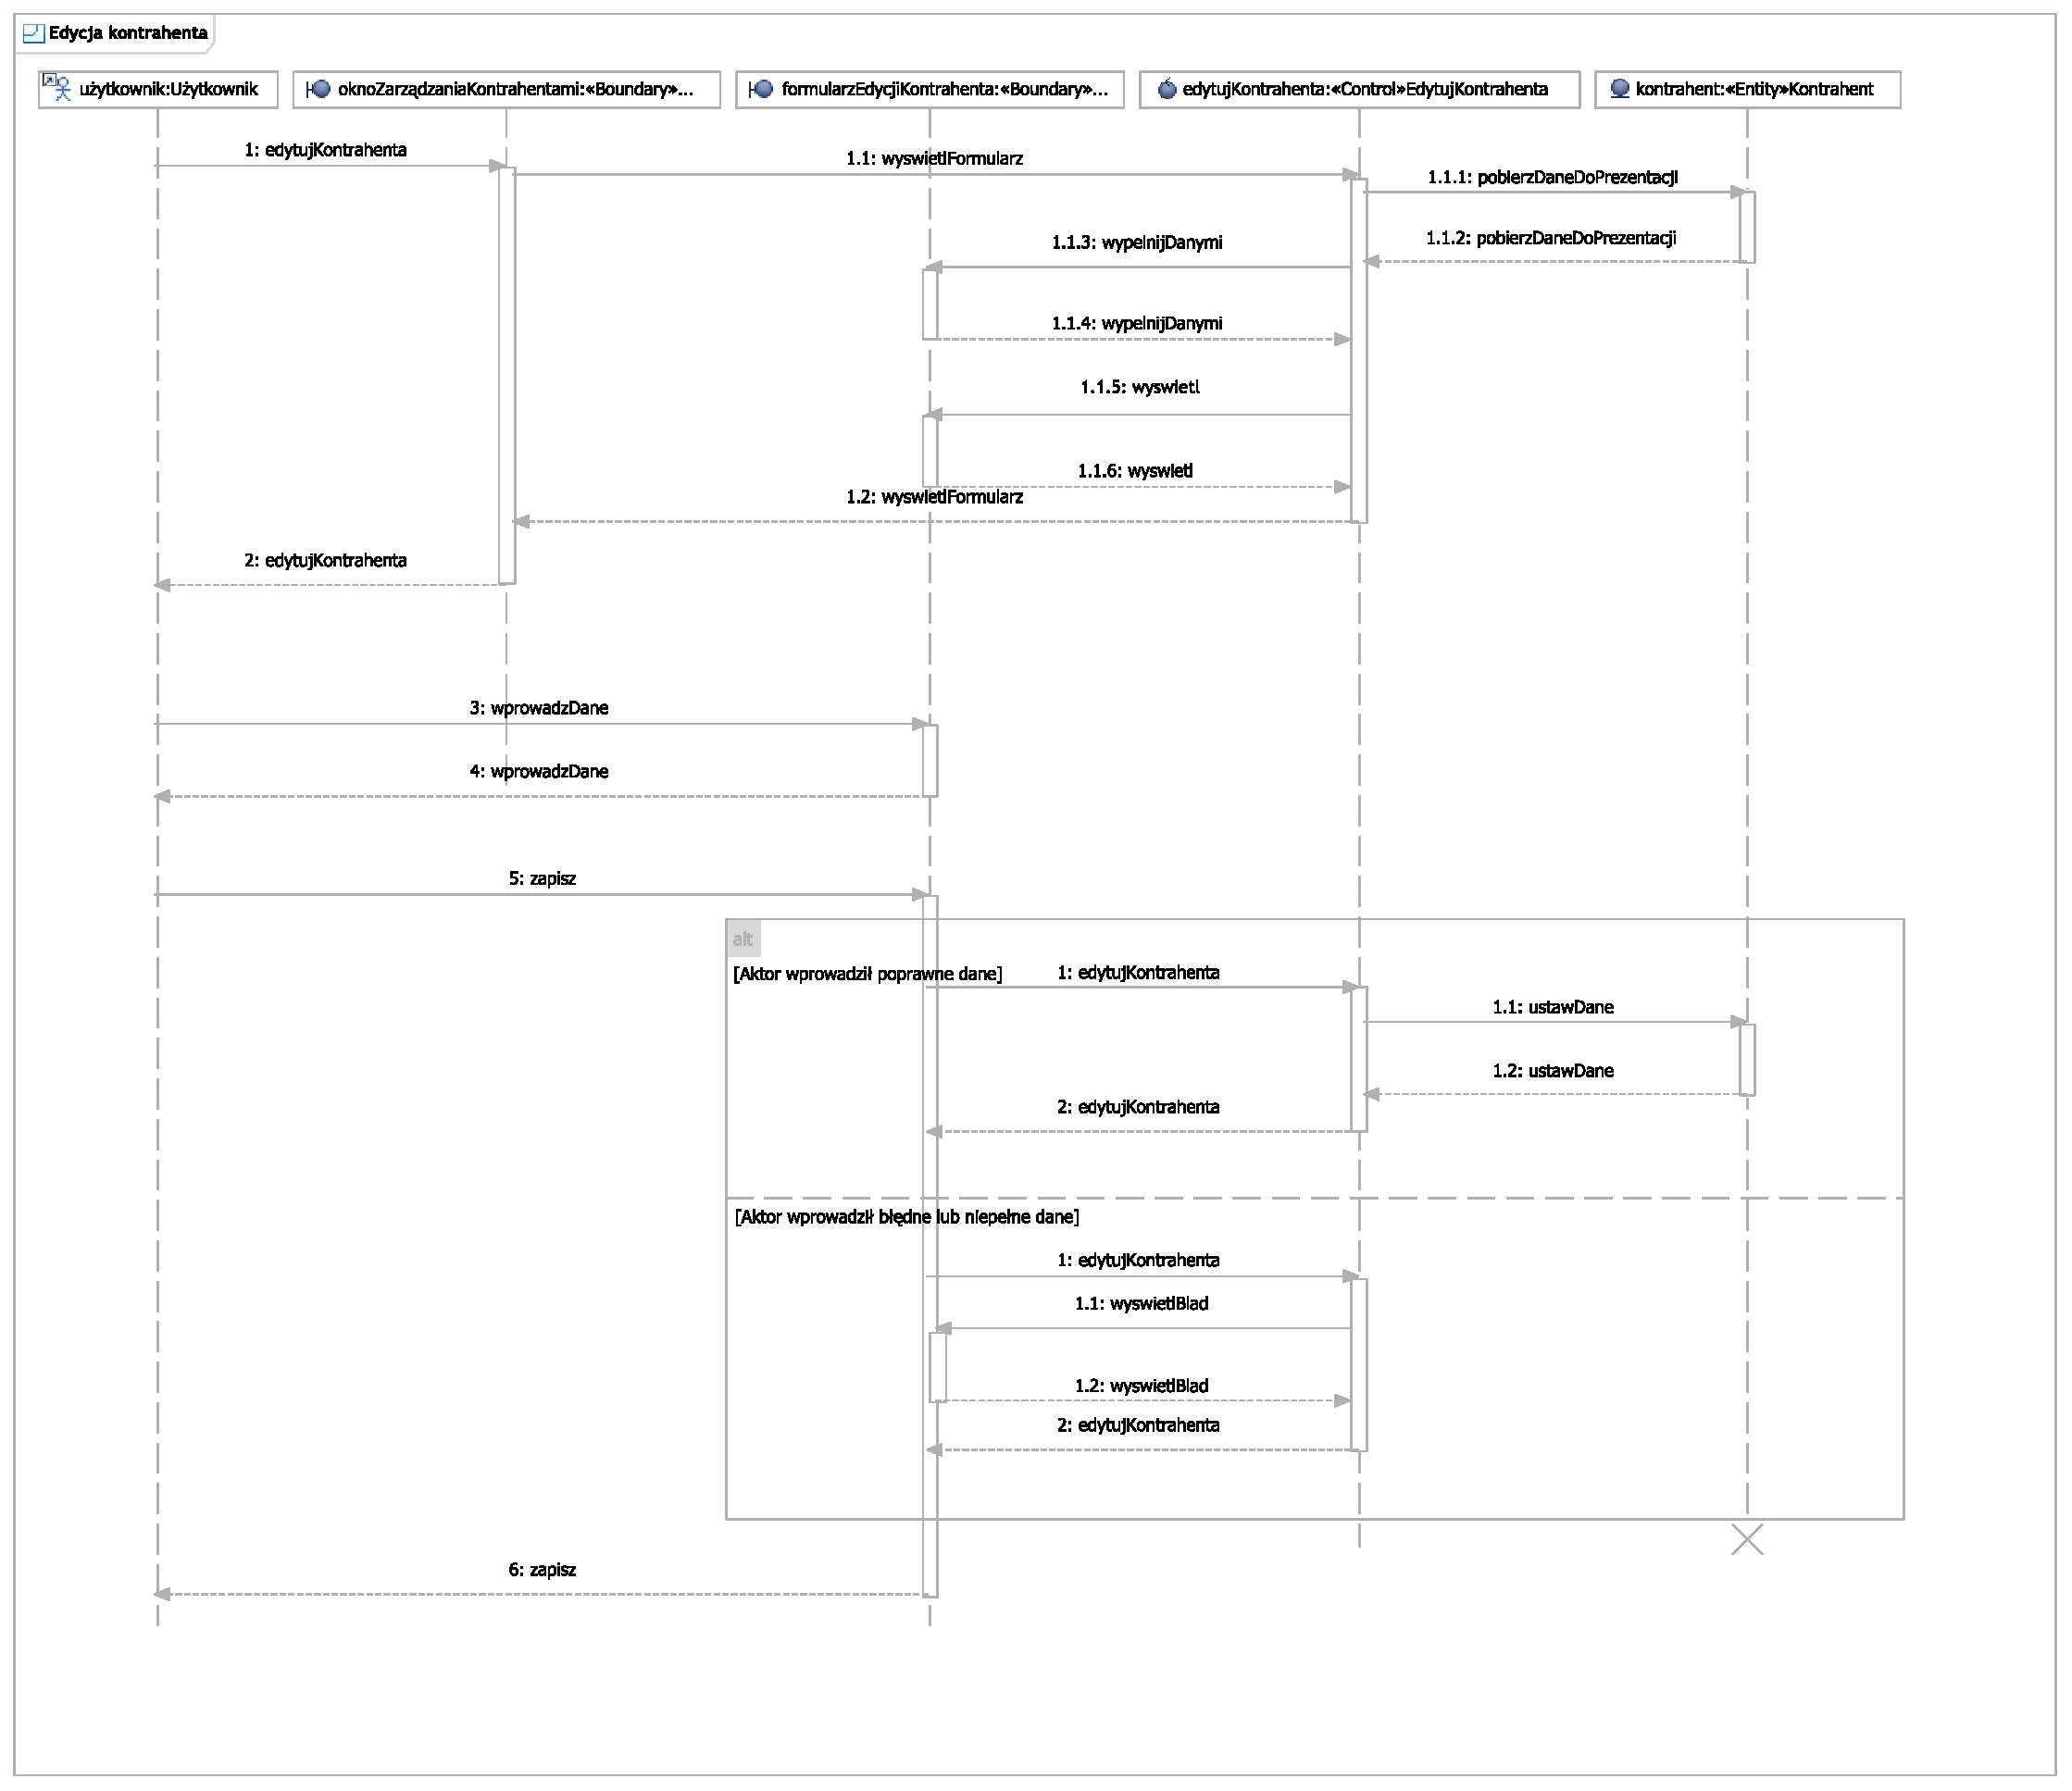
\includegraphics[angle=\seqangle, scale=0.43]{../img/usecase/pu10seq.pdf}
  \caption{\seqcaption10}
\end{figure}
\newpage

\subsection{Usuwanie danych kontrahentów}
\begin{usecase}
\addtitle{PU11}{Usuwanie danych kontrahenta} 
\addfield{Priorytet:}{wysoki}
\addfield{Aktor główny:}{Użytkownik}
\addfield{Rozszerza przypadki:}{PU8}
\additemizedfield{Warunki początkowe:}{
  \item Aktor został uwierzytelniony.
  \item W istnieje co najmniej jeden kontrahent.
} 
\addfield{Warunki końcowe:}{Dane kontrahenta zostają usunięte z systemu.}
\addscenario{Scenariusz główny:}{
	\item Aktor wybiera opcję usunięcia kontrahenta.
    \item System wyświetla okno potwierdzenia.
    \item Aktor zatwierdza usunięcie kontrahenta.
    \item System usuwa dane kontrahenta.
    \item System wyświetla potwierdzenie wykonania operacji.
}
\addscenario{Scenariusz alternatywny:}{
	\item[3.a] Aktor anuluje usuwanie kontrahenta.
		\begin{enumerate}
		\item[1.--2.] Jak w scenariuszu głównym.
		\item[3.] System zamyka okno potwierdzenia.
		\end{enumerate}
}
\addfield{Wymagania funkcjonalne}{3. Zarządzanie danymi kontrahentów, 3.3 Usuwanie danych kontrahentów}
\end{usecase}

\begin{figure}[H]
  \centering
  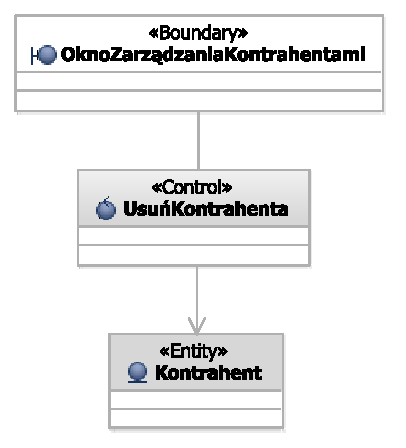
\includegraphics[angle=\ecbangle, scale=\ecbscale]{../img/usecase/pu11ecb.pdf}
  \caption{\ecbcaption11}
\end{figure}
\begin{figure}[H]
  \centering
  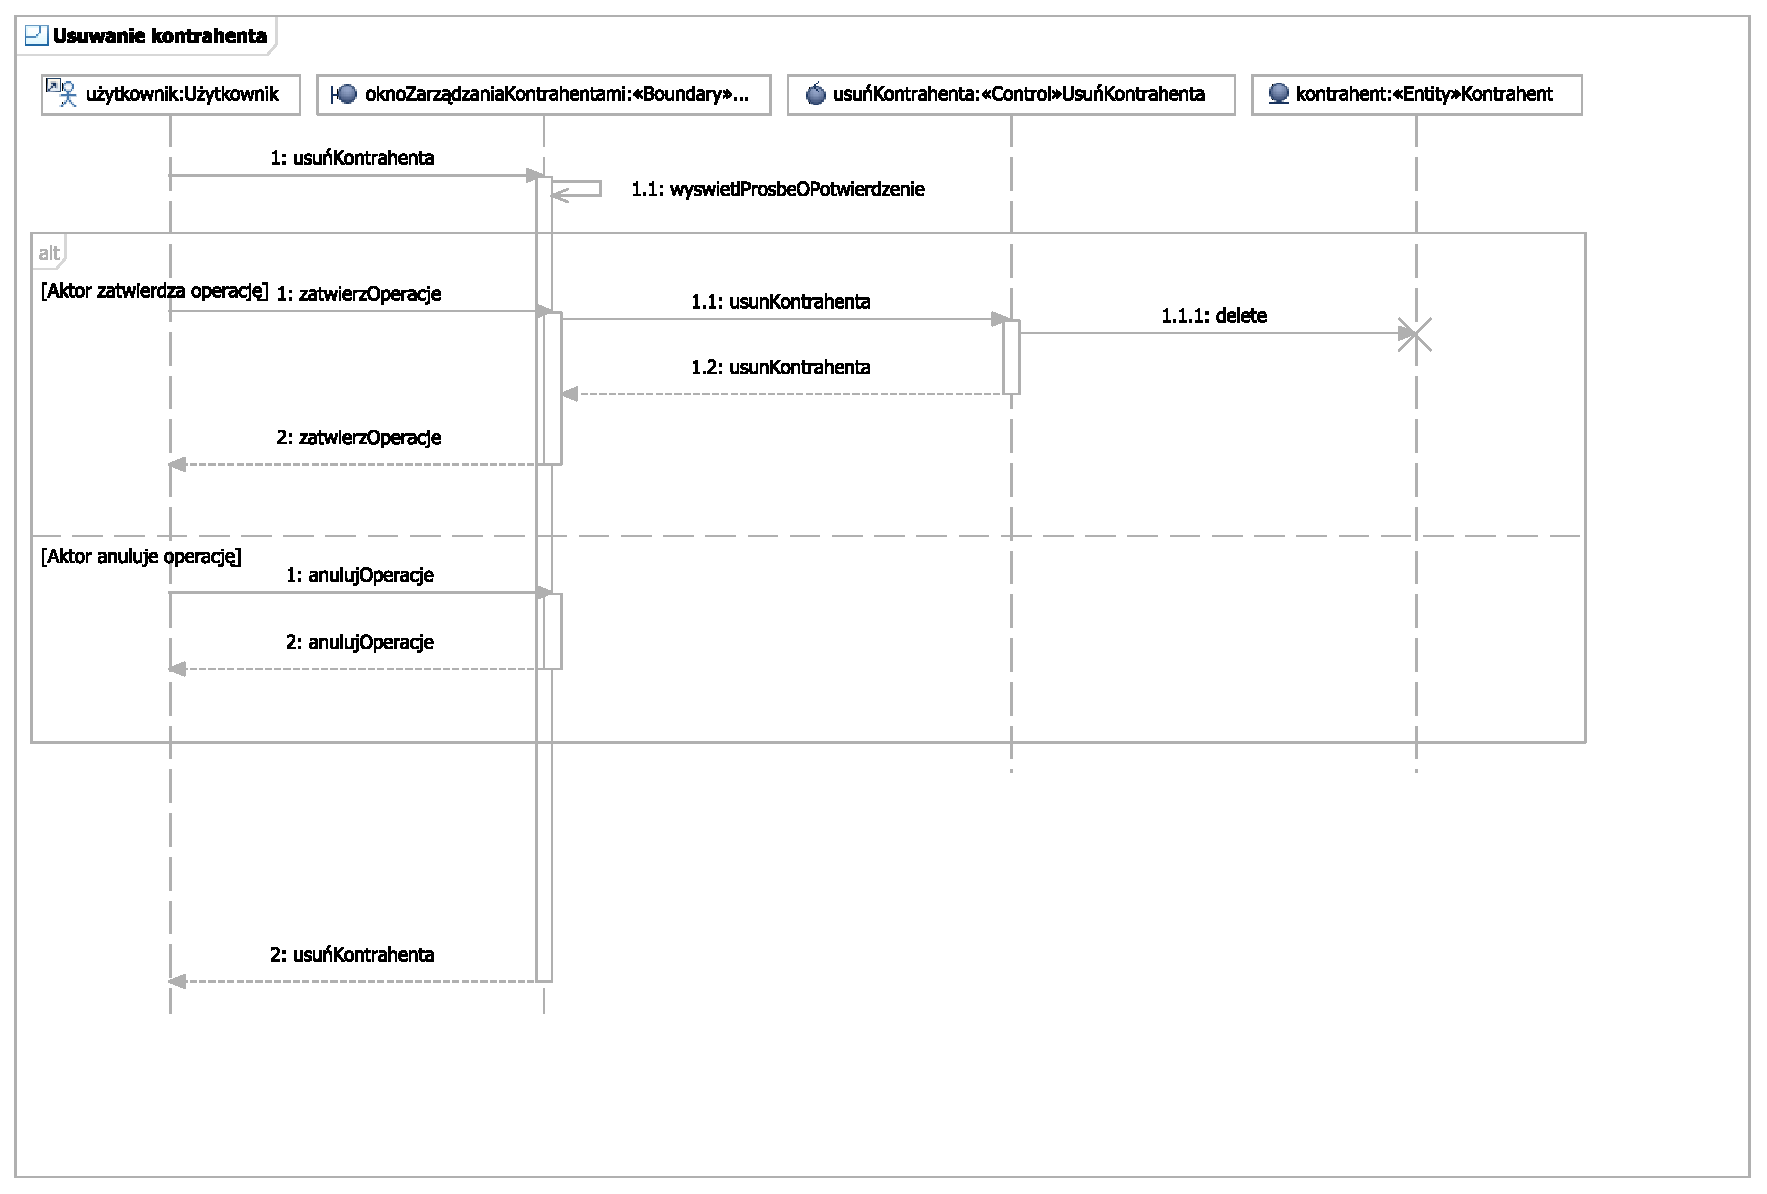
\includegraphics[angle=\seqangle, scale=0.55]{../img/usecase/pu11seq.pdf}
  \caption{\seqcaption11}
\end{figure}
\newpage
